\begin{figure}[t]
\centering
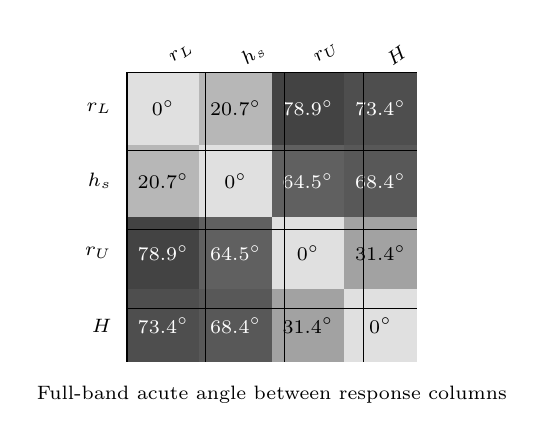
\begin{tikzpicture}[x=0.92cm,y=0.92cm]
\def\vals{
0/0/0,
1/0/20.7,
2/0/78.9,
3/0/73.4,
0/1/20.7,
1/1/0,
2/1/64.5,
3/1/68.4,
0/2/78.9,
1/2/64.5,
2/2/0,
3/2/31.4,
0/3/73.4,
1/3/68.4,
2/3/31.4,
3/3/0}
\foreach \x/\y/\v in \vals {
  \pgfmathsetmacro{\pct}{12+0.78*\v}
  \fill[black!\pct] (\x,-\y) rectangle ++(1,-1);
  \pgfmathparse{\v>55 ? "white" : "black"}
  \edef\txtcolor{\pgfmathresult}
  \node[text=\txtcolor,font=\scriptsize] at (\x+0.5,-\y-0.5) {\v$^\circ$};
}
\draw (0,0) grid (4,-4);
\foreach \x/\lab in {0/$r_L$,1/$h_s$,2/$r_U$,3/$H$}
  \node[font=\scriptsize,rotate=35,anchor=west] at (\x+0.5,0.08) {\lab};
\foreach \y/\lab in {0/$r_L$,1/$h_s$,2/$r_U$,3/$H$}
  \node[font=\scriptsize,anchor=east] at (-0.08,-\y-0.5) {\lab};
\node[font=\scriptsize] at (2,-4.45) {Full-band acute angle between response columns};
\end{tikzpicture}
\caption{Pairwise acute angles between the four full-band geometry-response columns. Large angles indicate controls that act in substantially different directions. The $78.9^\circ$ separation between $r_L$ and $r_U$ is the key evidence that splitting the post creates a non-redundant control direction.}
\label{fig:angle-matrix}
\end{figure}
